\documentclass[11pt,a4paper]{article}
\usepackage[margin=1in]{geometry}
\usepackage{amsmath,graphicx,booktabs,float,hyperref,enumitem,array}
\usepackage{times}
\hypersetup{colorlinks=true,linkcolor=blue,urlcolor=blue}
\graphicspath{{diagrams/}}
\begin{document}
\begin{titlepage}\centering\vspace*{2cm}
{\Large Mawlana Bhashani Science and Technology University\par}
{\large Department of Information and Communication Technology\par}\vspace{1.5cm}
{\large Course Title: Software Development and Project Management\par}\vspace{.2cm}{\large Course Code: ICT 3108\par}\vspace{1cm}
{\Huge\bfseries StockPilot\par}\vspace{.3cm}
{\Large Intelligent Inventory and Business Analytics System\par}\vspace{.5cm}
{\large Part I --- Final Capstone Project Proposal and Prototyping\par}\vspace{2cm}
\begin{tabular}{rl}
Student Name: & \textbf{Samiul Islam}\\
Student ID: & \textbf{IT24011}\\
GitHub: & \url{https://github.com/SAMIUL-01/StockPilot}\\
\end{tabular}
\end{titlepage}
\tableofcontents\newpage

\begin{abstract}
Small retail shops in Bangladesh usually track stock in notebooks or spreadsheets. This causes stock-outs, expired or dead stock, and no clear view of profit. \textbf{StockPilot} is an inventory management system that goes beyond storing stock counts. It records every stock movement, calculates gross profit per sale, and gives rule-based \emph{Smart Restock} advice explaining what to reorder, how much, and why. This proposal presents the problem, objectives, scope, requirements, process model, schedule with Gantt chart, six UML diagrams, and a working Java prototype with a simple Swing interface built from seven classes.
\end{abstract}

\section{Introduction and Background}
Inventory is the largest working asset of a small retail business. Wrong stock decisions either tie up money (over-stocking) or lose sales (stock-outs). Existing commercial systems are expensive or too complex for small shops. StockPilot targets a low-cost, easy-to-use system that turns daily sales data into reorder decisions.

\section{Problem Statement}
\begin{itemize}[noitemsep]
\item Stock is tracked manually, so counts are often wrong.
\item Owners only notice low stock after a product has run out.
\item Profit per product is unknown because cost and selling price are not linked to each sale.
\item There is no history of who changed stock, when, and why.
\end{itemize}

\section{Aim and Objectives}
\textbf{Aim:} to design and prototype an inventory system that supports daily operations and recommends restocking decisions.
\begin{enumerate}[noitemsep]
\item Manage products, categories and suppliers with validated data.
\item Process sales with automatic invoice calculation and stock deduction.
\item Maintain a complete audit trail of every stock movement.
\item Compute gross profit and margin from cost snapshots stored with each sale.
\item Recommend reorder quantity using sales history and supplier lead time.
\item Provide a dashboard showing KPIs and low-stock alerts.
\end{enumerate}

\section{Proposed System and Unique Features}
\begin{description}[noitemsep]
\item[Smart Restock Advisor] Reorder point $=\lceil \text{avg daily sales}\times\text{lead time}\rceil+\text{safety stock}$. If current stock is below it, the system suggests an order quantity and prints the reason. Example: average 5/day, lead time 4 days, safety stock 8 gives reorder point 28; with stock 12 an alert is raised.
\item[Profit Intelligence] Each sale line stores a price and cost snapshot, so profit stays correct when prices change later.
\item[Stock Movement Audit Trail] Every stock-in, sale and adjustment is logged with time, type, quantity and reason.
\item[All-or-nothing billing] A sale is validated completely before any stock is deducted; insufficient stock rejects the whole invoice.
\item[Expiry and dead-stock reports] Planned for the full version.
\end{description}

\section{Scope and Target Users}
\textbf{In scope (prototype):} product management, sales and billing, low-stock alerts, restock advice, audit trail, dashboard. \textbf{Planned (full version):} purchases, supplier management, user roles, reports export, expiry tracking. \textbf{Out of scope:} online payment, e-commerce integration, multi-branch support. \textbf{Users:} Admin (shop owner/manager) and Staff (sales counter).

\section{Requirements}
\subsection{Functional Requirements}
\begin{enumerate}[noitemsep,label=FR\arabic*.]
\item The system shall allow Admin to add products with unique SKU, cost, price, opening stock and reorder level.
\item The system shall allow Staff to build a cart and complete a sale.
\item The system shall reject a sale if any item exceeds available stock.
\item The system shall deduct stock and log a movement for every sale.
\item The system shall flag products whose stock is at or below reorder level.
\item The system shall show restock suggestions with quantity and reason.
\item The system shall calculate total sales and gross profit.
\item The system shall support role-based login (full version).
\end{enumerate}
\subsection{Non-functional Requirements}
\textbf{Usability:} simple dashboard, usable without training. \textbf{Reliability:} no negative stock; stock and sale updated together. \textbf{Performance:} actions respond within one second for up to 10,000 products. \textbf{Maintainability:} separate classes with single responsibilities. \textbf{Security:} hashed passwords and role-based access (full version). \textbf{Portability:} runs on any system with JDK 21.

\section{Technology Stack and Architecture}
\begin{table}[H]\centering\begin{tabular}{ll}\toprule
\textbf{Layer} & \textbf{Technology}\\\midrule
Prototype UI & Java Swing (JDK 21)\\
Business logic & Plain Java (OOP), packages \texttt{stockpilot}\\
Full-version backend & Java, Spring Boot, Maven (REST API)\\
Full-version frontend & HTML, CSS, JavaScript, Chart.js\\
Database & MySQL (prototype uses in-memory collections)\\
Tools & Git/GitHub, diagrams.net, Graphviz, JUnit, Overleaf\\\bottomrule
\end{tabular}\end{table}
The prototype follows a layered design: UI (\texttt{MainApp}) $\rightarrow$ service layer (\texttt{InventoryService}, \texttt{RestockAdvisor}) $\rightarrow$ domain classes (\texttt{Product}, \texttt{Sale}, \dots).

\section{Software Process Model}
\textbf{Selected model: Agile (Scrum-style incremental development).} Requirements are clear at a high level but details (reports, restock rules) will change after feedback, so short iterations suit the project better than a rigid Waterfall plan. Work is divided into sprints, each ending with a working increment.
\begin{table}[H]\centering\begin{tabular}{llp{6cm}}\toprule
\textbf{Sprint} & \textbf{Period} & \textbf{Goal}\\\midrule
Sprint 0 & 18--21 Oct & Requirements, design, UML, repository setup\\
Sprint 1 & 22--24 Oct & Core classes, sales workflow, Swing interface\\
Sprint 2 & 25--27 Oct & Testing, screenshots, report, submission\\\bottomrule
\end{tabular}\end{table}
After submission, further sprints add purchases, user roles, Spring Boot API with MySQL, reports and deployment.

\section{Schedule, Milestones and Deliverables}
\begin{table}[H]\centering\small\begin{tabular}{llp{5.2cm}}\toprule
\textbf{Task} & \textbf{Dates (2026)} & \textbf{Deliverable}\\\midrule
Scope and requirements & 18 Oct & Requirement list (M1)\\
Proposal draft & 19--20 Oct & Proposal sections\\
UML and database design & 19--21 Oct & Six diagrams, ERD (M2)\\
Project setup, class design & 21 Oct & GitHub repo, class skeleton\\
Core classes & 22--23 Oct & Working domain and service code (M3)\\
Swing prototype & 23--24 Oct & Dashboard and workflow screens\\
Testing and screenshots & 25 Oct & Test results, screenshots (M4)\\
Report finalization & 25--26 Oct & Final PDF, README\\
Review and submission & 27 Oct & Repository URL on Canvas (M5)\\\bottomrule
\end{tabular}\end{table}
\begin{figure}[H]\centering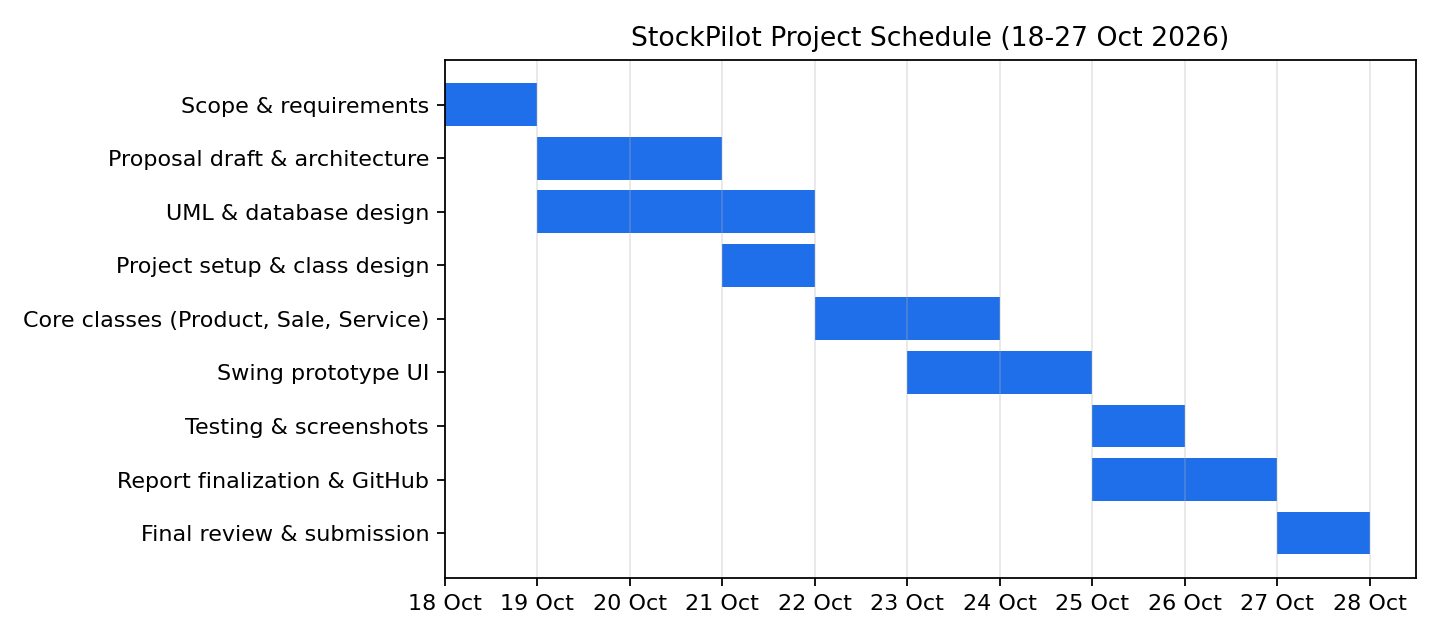
\includegraphics[width=.95\textwidth]{gantt.png}\caption{Gantt chart}\end{figure}

\section{UML Diagrams}
\subsection{Data Flow Diagram}
Admin, Staff and Supplier interact with five processes and four data stores. Sales deduct stock and write stock movements; the restock advisor reads sales history and stock.
\begin{figure}[H]\centering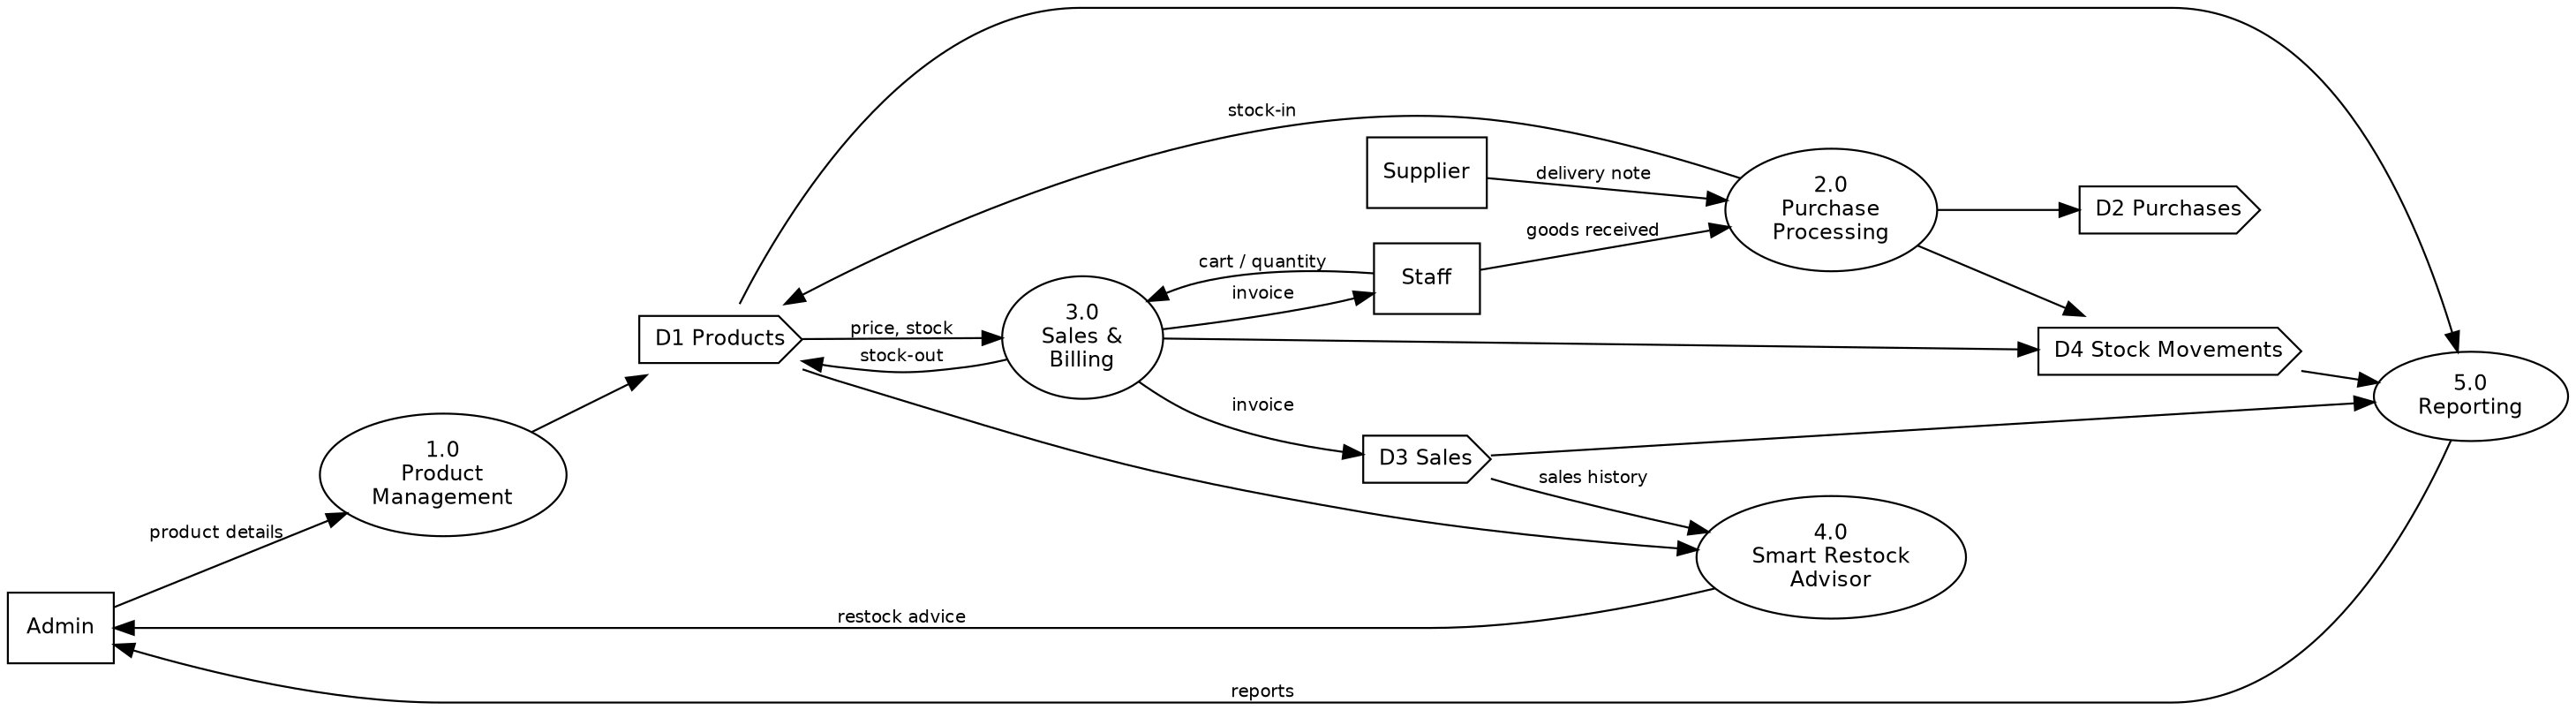
\includegraphics[width=\textwidth]{dfd.png}\caption{Data flow diagram}\end{figure}
\subsection{Use Case Diagram}
Admin manages products, suppliers, users and views reports; Staff records purchases and processes sales.
\begin{figure}[H]\centering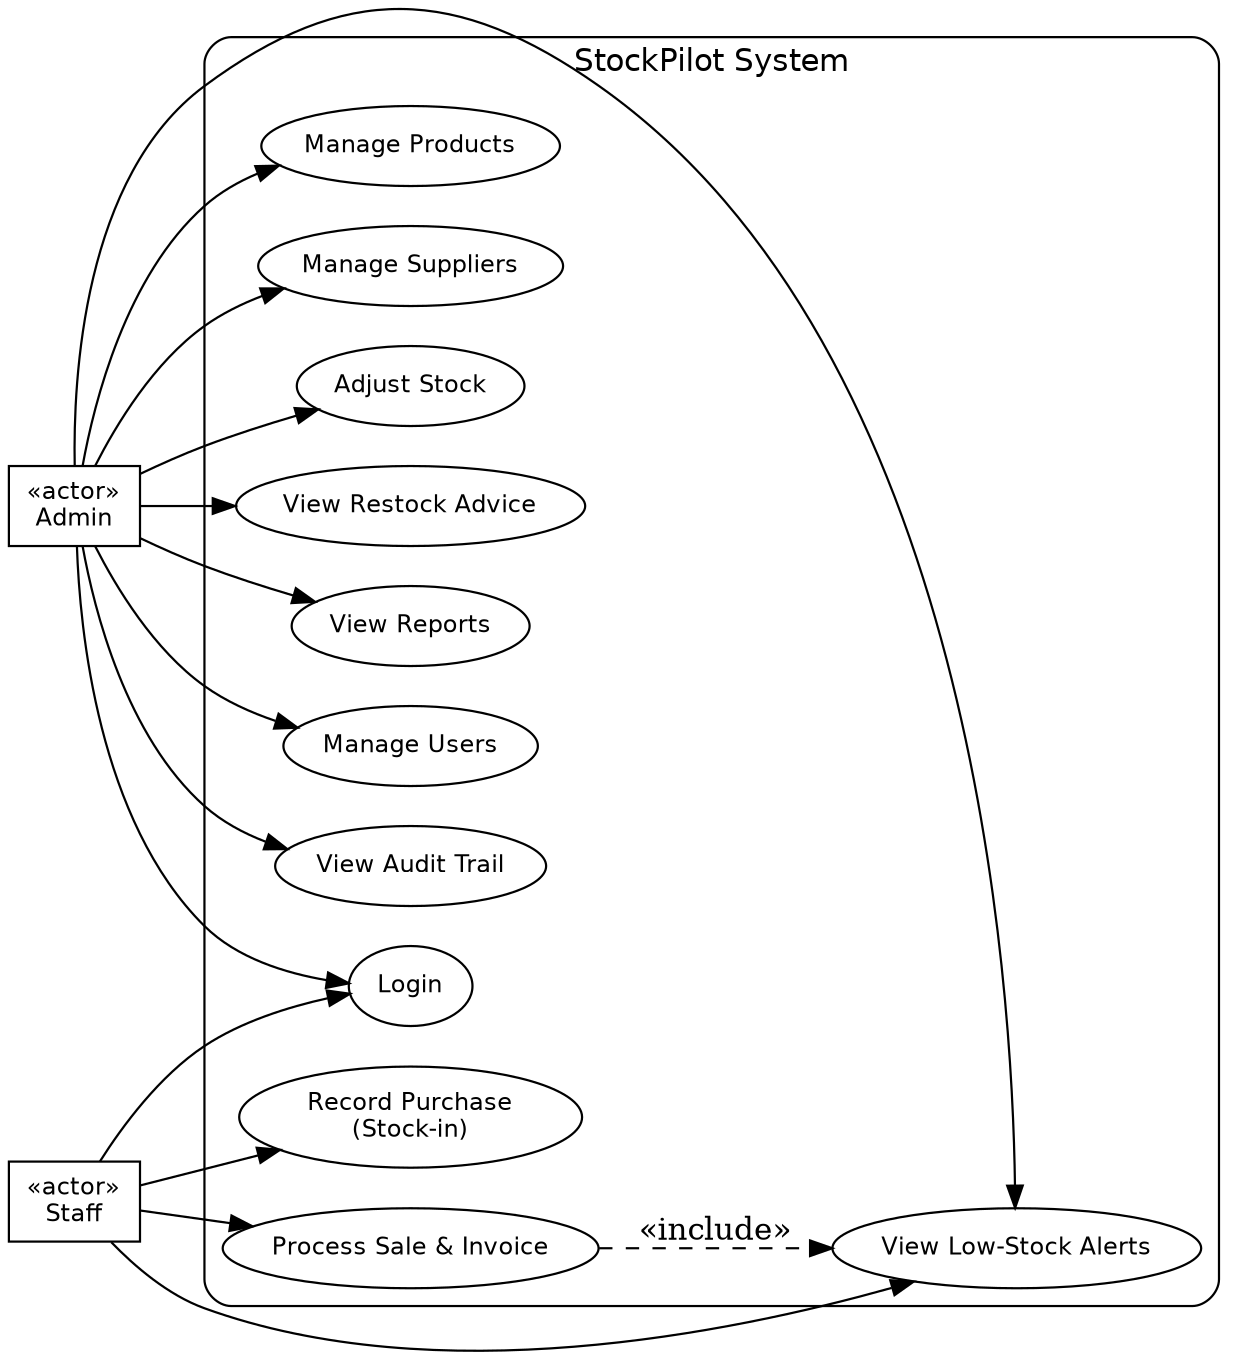
\includegraphics[width=.85\textwidth]{usecase.png}\caption{Use case diagram}\end{figure}
\subsection{Activity Diagram}
The sales workflow, including the error branch for insufficient stock.
\begin{figure}[H]\centering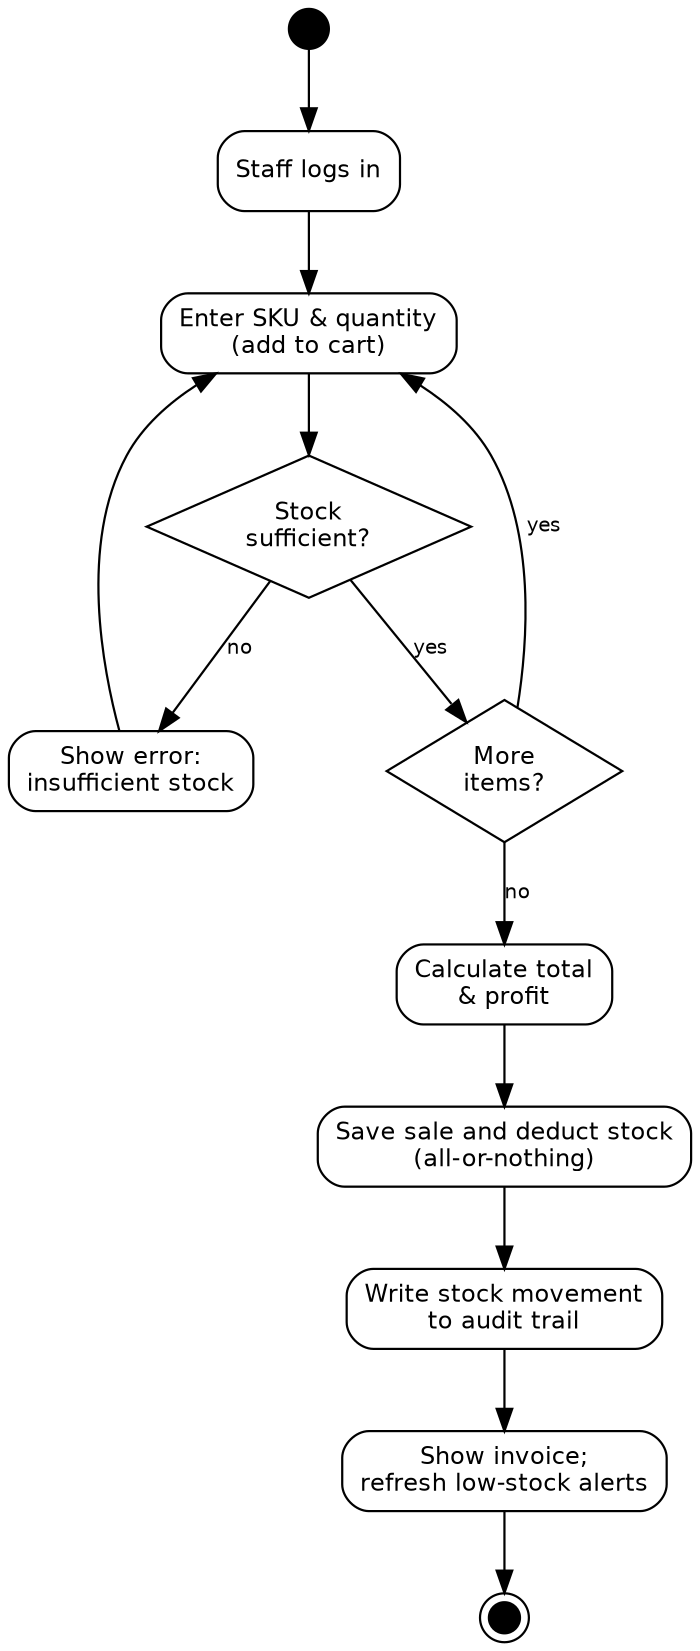
\includegraphics[height=.55\textheight]{activity.png}\caption{Activity diagram: sales and billing}\end{figure}
\subsection{Entity Relationship Diagram}
Nine tables for the full version; \texttt{stock\_movements} records every stock change.
\begin{figure}[H]\centering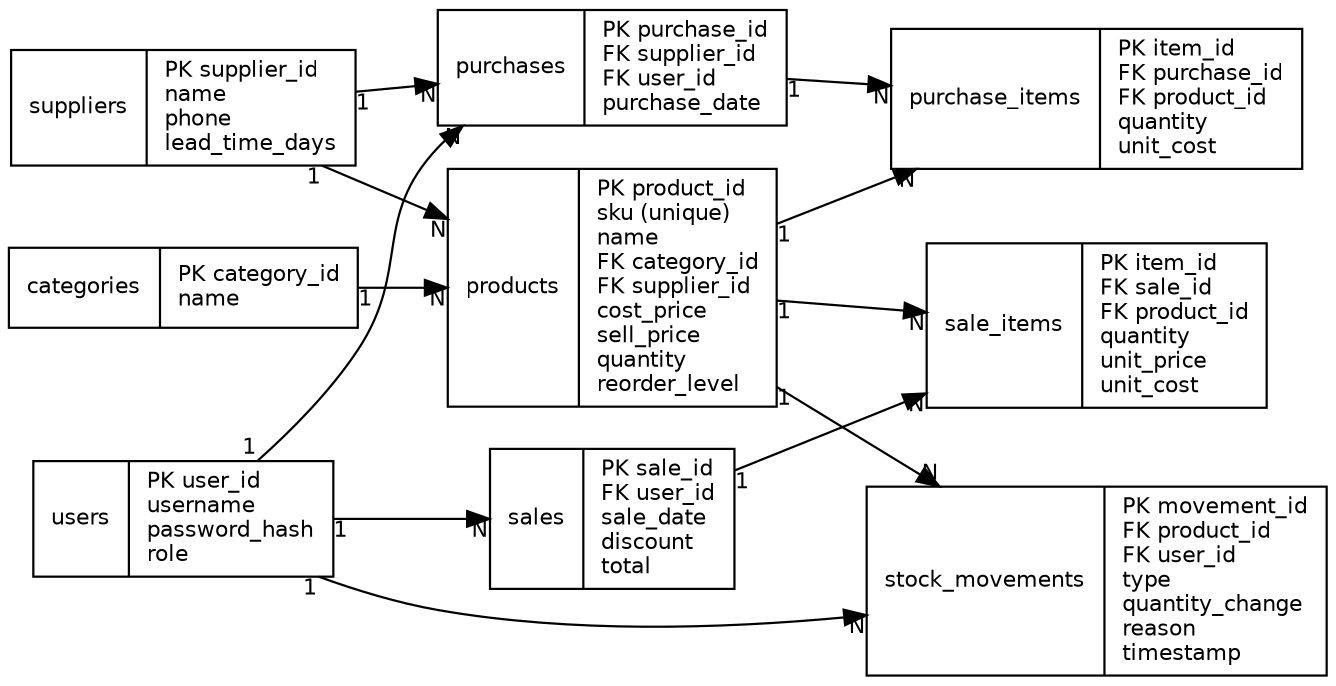
\includegraphics[width=\textwidth]{erd.png}\caption{Entity relationship diagram}\end{figure}
\subsection{Class Diagram}
The prototype implements these classes: \texttt{Category}, \texttt{Supplier}, \texttt{Product}, \texttt{SaleItem}, \texttt{Sale}, \texttt{InventoryService}, \texttt{RestockAdvisor}, \texttt{InsufficientStockException} and the UI class \texttt{MainApp}.
\begin{figure}[H]\centering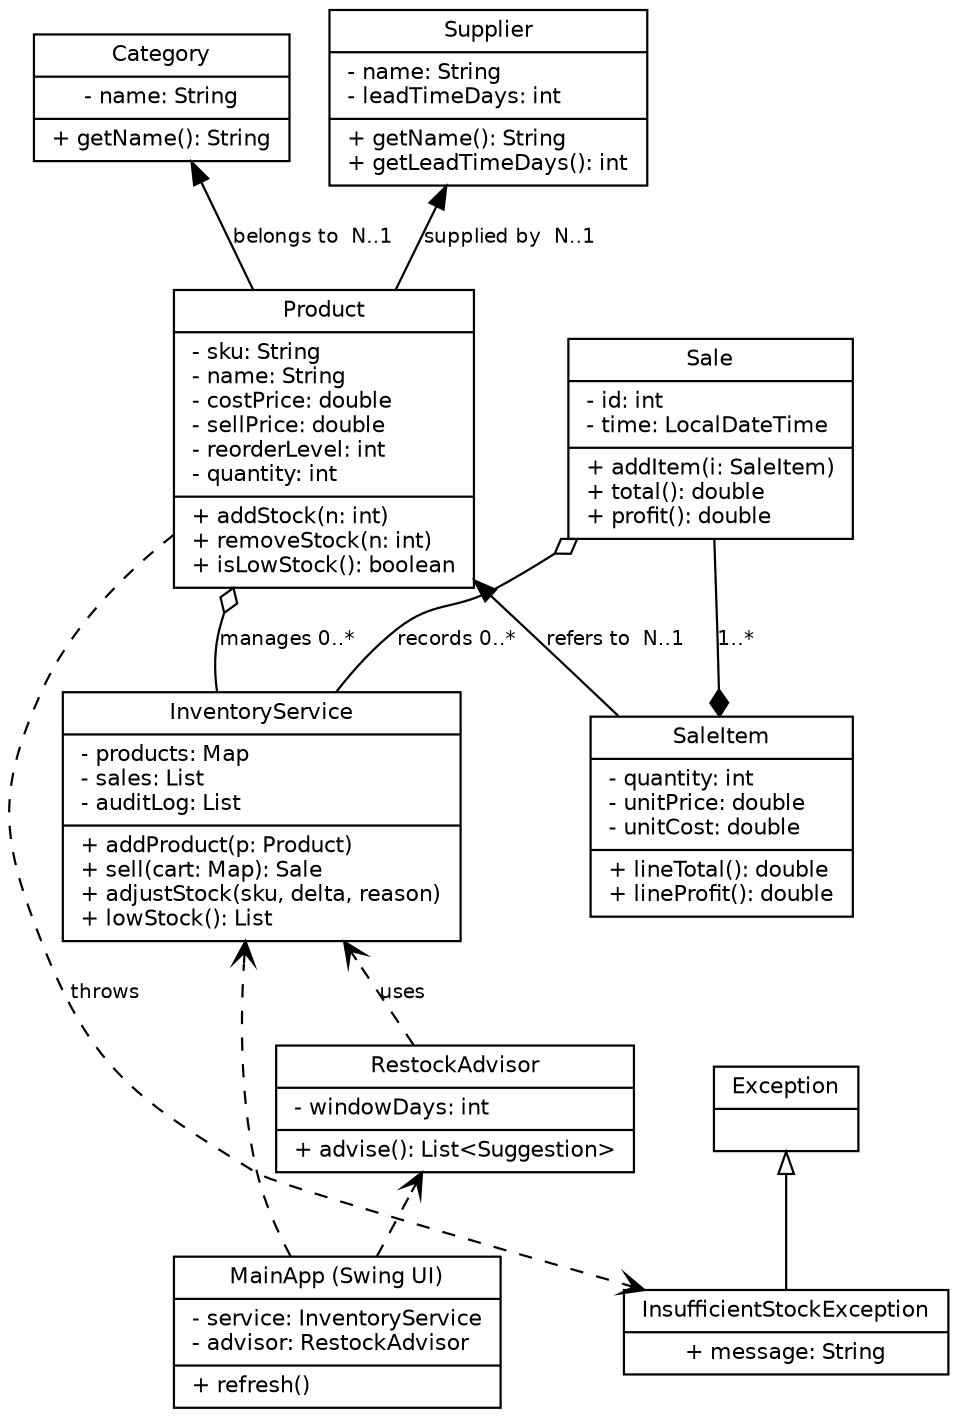
\includegraphics[height=.62\textheight]{class.png}\caption{Class diagram}\end{figure}
\textbf{OOP concepts used:} encapsulation (private \texttt{quantity} changed only through validated methods), composition (\texttt{Sale} contains \texttt{SaleItem}s), inheritance (custom exception extends \texttt{Exception}), exception handling (rejecting oversized sales), and abstraction through the service layer.
\subsection{Object Diagram}
A snapshot of sample objects at run time.
\begin{figure}[H]\centering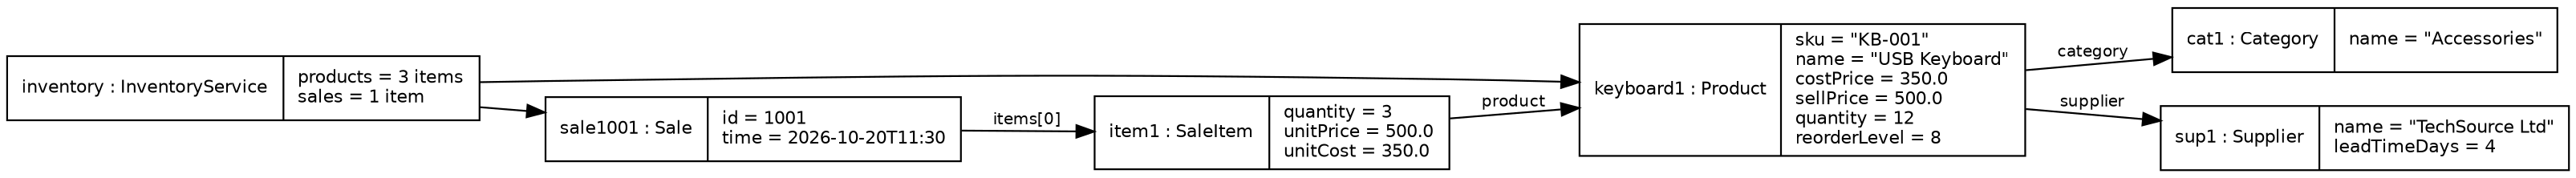
\includegraphics[width=\textwidth]{object.png}\caption{Object diagram}\end{figure}

\section{Prototype}
The prototype is a Java Swing desktop application in \texttt{src/main/java/stockpilot}. It uses seven domain/service classes plus the UI. Tabs: \textbf{Dashboard} (product count, sales, low-stock count, gross profit), \textbf{Products} (table and add form with validation), \textbf{Sales and Billing} (cart, checkout, invoice), \textbf{Smart Restock} (suggestions with reasons), \textbf{Audit Trail}. Data is held in memory; database persistence is planned. Run instructions are in the README.

% Add screenshots here after running the app:
% \begin{figure}[H]\centering\includegraphics[width=.9\textwidth]{../screenshots/dashboard.png}\caption{Dashboard}\end{figure}

\section{Testing Plan and Expected Outcomes}
\begin{table}[H]\centering\small\begin{tabular}{lp{5.5cm}p{4.5cm}}\toprule
\textbf{Test} & \textbf{Input} & \textbf{Expected result}\\\midrule
Add product & Valid SKU, prices, stock & Product listed, audit entry added\\
Duplicate SKU & Existing SKU & Error message\\
Valid sale & KB-001 $\times$ 3 & Stock reduced by 3, invoice shown\\
Oversized sale & KB-001 $\times$ 100 & Rejected, stock unchanged\\
Low-stock alert & Stock $\le$ reorder level & Product marked LOW\\
Restock advice & Stock below reorder point & Suggestion with reason\\\bottomrule
\end{tabular}\end{table}
Expected outcome: a working, validated inventory workflow that demonstrates the design and can be extended into the full system.

\section{Limitations and Future Enhancements}
The prototype stores data in memory, so it resets on exit; login, purchases, expiry alerts, exports and the Spring Boot/MySQL backend are future work. Restock advice uses simple averages and does not yet consider seasonality or pending orders.

\begin{thebibliography}{9}
\bibitem{sommerville} I. Sommerville, \emph{Software Engineering}, 10th ed., Pearson, 2016.
\bibitem{fowler} M. Fowler, \emph{UML Distilled}, 3rd ed., Addison-Wesley, 2003.
\bibitem{schwaber} K. Schwaber and J. Sutherland, \emph{The Scrum Guide}, 2020.
\bibitem{oracle} Oracle, \emph{Java SE Documentation}, \url{https://docs.oracle.com/en/java/}.
\end{thebibliography}

\section*{GitHub Repository}
\url{https://github.com/SAMIUL-01/StockPilot}
\end{document}
